\chapter{第一个电路}\label{ch:g3:first-electric-circuit}

咔哒一声——手电筒把光束射过黑暗的房间。塑料筒里
住着一节\omterm{def:g3:first-electric-circuit:battery}{电池}、一个小\omterm{def:g3:first-electric-circuit:bulb}{灯泡}和两片金属片，
它们正在玩一场规则严格的游戏。今天我们就来拆开这个游戏：
只用一节\omterm{def:g3:first-electric-circuit:battery}{电池}、一个\omterm{def:g3:first-electric-circuit:bulb}{灯泡}和两根导线，
我们就能亲手让灯亮起来。

\section{灯泡、电池与两根导线}

\begin{definition}[电池]\label{def:g3:first-electric-circuit:battery}
称\emph{电池}\index{电池}为一个小小的电的储存器。它
有两个不同的端，叫作它的
\emph{接线柱}\index{接线柱}：一端标 $+$，
另一端标 $-$。两端都很重要，
只有两端都接入时，电才会参与这场游戏。
\end{definition}

\begin{definition}[灯泡]\label{def:g3:first-electric-circuit:bulb}
称\emph{灯泡}\index{灯泡}为一种小灯，玻璃壳内装有一根细细的灯丝，
当电流流过时，它会白炽发光。
仔细看它的金属底座：灯泡同样有\emph{两个}
接触点——最底下的尖端，以及金属底座的侧面。
\omterm{def:g3:first-electric-circuit:battery}{电池}有两个\omterm{def:g3:first-electric-circuit:battery}{接线柱}，灯泡有两个接触点：
这绝非巧合。
\end{definition}

\begin{method}[点亮灯泡]\label{met:g3:first-electric-circuit:light}
用一节\omterm{def:g3:first-electric-circuit:battery}{电池}、一个\omterm{def:g3:first-electric-circuit:bulb}{灯泡}和两根导线：
\begin{enumerate}
  \item 用一根导线把\omterm{def:g3:first-electric-circuit:battery}{电池}的 $+$ \omterm{def:g3:first-electric-circuit:battery}{接线柱}接到
        \omterm{def:g3:first-electric-circuit:bulb}{灯泡}底座的尖端；
  \item 用另一根导线把\omterm{def:g3:first-electric-circuit:battery}{电池}的 $-$ \omterm{def:g3:first-electric-circuit:battery}{接线柱}接到
        \omterm{def:g3:first-electric-circuit:bulb}{灯泡}底座的金属侧面；
  \item \omterm{def:g3:first-electric-circuit:bulb}{灯泡}亮了——你已经搭成了一个\omterm{def:g3:first-electric-circuit:circuit}{电路}！
\end{enumerate}
如果灯还是不亮，先检查这几个常见原因：导线碰到了
玻璃而不是金属接触点，连接松动，
或者\omterm{def:g3:first-electric-circuit:battery}{电池}用旧了。
\end{method}

\begin{omfigure}
\begin{tikzpicture}[scale=0.85]
  \draw[thick, fill=omExo, fill opacity=0.2] (0,0.4) rectangle (1.7,3.0);
  \draw[thick] (0.55,3.0) rectangle (1.15,3.35);
  \node[font=\small] at (0.85,1.7) {电池};
  \node[font=\footnotesize] at (0.85,3.17) {$+$};
  \node[font=\footnotesize] at (0.85,0.65) {$-$};
  \draw[thick] (5.8,2.6) circle (0.75);
  \draw[thick] (5.45,2.0) -- (5.45,1.5) -- (6.15,1.5) -- (6.15,2.0);
  \draw[thick] (5.6,1.5) -- (5.6,1.1) (6.0,1.5) -- (6.0,1.1)
    (5.6,1.1) -- (6.0,1.1);
  \draw[thick] (5.62,2.35) .. controls (5.75,2.6) .. (5.8,2.35)
    .. controls (5.85,2.6) .. (5.98,2.35);
  \node[right, font=\small] at (6.8,2.7) {带发光灯丝的玻璃};
  \node[right, font=\small] at (6.8,1.7) {金属底座：侧面接触};
  \node[right, font=\small] at (6.8,1.0) {底部尖端接触};
  \draw[-Stealth, omExo] (6.7,1.05) -- (5.85,1.05);
  \draw[thick, omThm] (0.85,3.35) -- (0.85,4.0) -- (5.8,4.0)
    -- (5.8,3.35);
  \draw[thick, omDef] (0.85,0.4) -- (0.85,-0.3) -- (5.8,-0.3)
    -- (5.8,1.1);
  \node[above, font=\small, omThm] at (3.3,4.05)
    {导线：接 $+$ 到尖端？不对——应接任一接触点};
\end{tikzpicture}

{\small 角色介绍：一节带两个\omterm{def:g3:first-electric-circuit:battery}{接线柱}的\omterm{def:g3:first-electric-circuit:battery}{电池}，一个带两个接触点的\omterm{def:g3:first-electric-circuit:bulb}{灯泡}，
以及连接它们的两根导线。}
\end{omfigure}

\begin{omfigure}
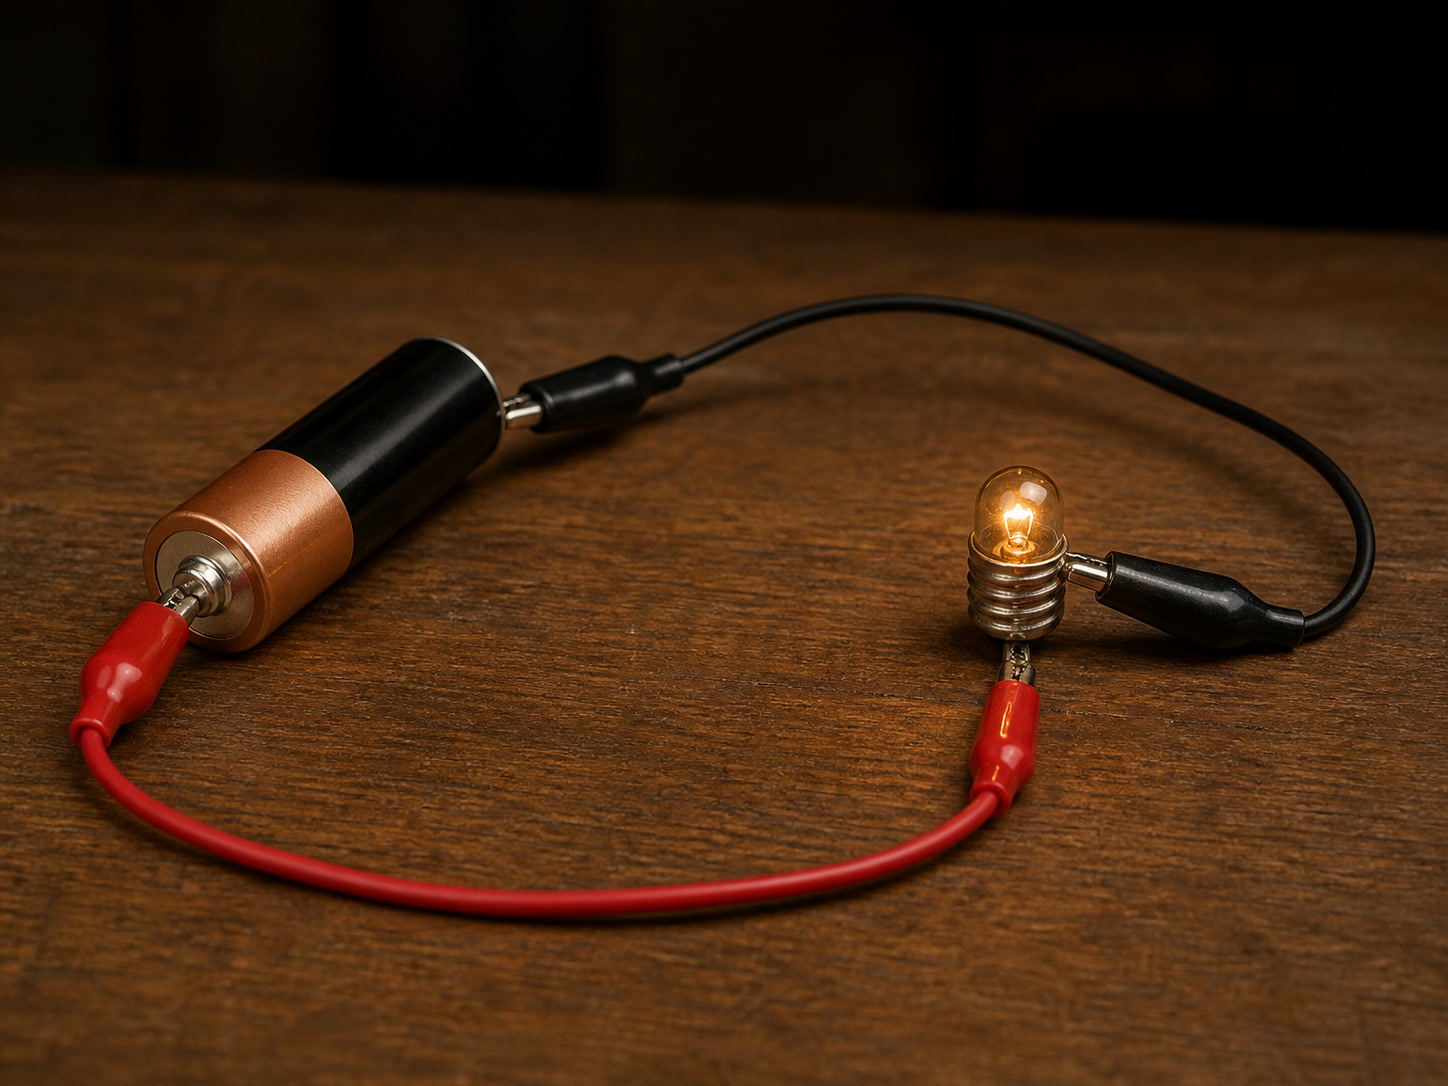
\includegraphics[width=0.5\linewidth]{images/book1/ai/g3-circuit-bulb.jpg}

{\small 回路闭合的那一刻：\omterm{def:g3:first-electric-circuit:battery}{电池}、两根导线，小\omterm{def:g3:first-electric-circuit:bulb}{灯泡}亮了起来。}
\end{omfigure}

\section{电路必须闭合}

\begin{definition}[电路]\label{def:g3:first-electric-circuit:circuit}
称\emph{电路}\index{电路}为一个供电流流通的完整回路：
电流从\omterm{def:g3:first-electric-circuit:battery}{电池}的一个\omterm{def:g3:first-electric-circuit:battery}{接线柱}出发，经过导线和\omterm{def:g3:first-electric-circuit:bulb}{灯泡}，
再回到另一个\omterm{def:g3:first-electric-circuit:battery}{接线柱}。当回路完整时，我们说
这个电路是
\emph{闭合电路}\index{闭合电路}；若其中某处有缺口，则它是
\emph{断开的电路}\index{断开的电路}。
\end{definition}

\begin{proposition}[回路定律]\label{prop:g3:first-electric-circuit:loop}
只有\omterm{def:g3:first-electric-circuit:circuit}{电路}闭合时\omterm{def:g3:first-electric-circuit:bulb}{灯泡}才会亮——也就是说，
从\omterm{def:g3:first-electric-circuit:battery}{电池}的一个\omterm{def:g3:first-electric-circuit:battery}{接线柱}出发，经过\omterm{def:g3:first-electric-circuit:bulb}{灯泡}，
再回到另一个\omterm{def:g3:first-electric-circuit:battery}{接线柱}，形成一个不间断的回路。
回路中哪怕只有一处缺口，\omterm{def:g3:first-electric-circuit:bulb}{灯泡}就会熄灭：电不会跨过缺口，
也不会流进死胡同。
\end{proposition}

\begin{example}[为什么要两端都接？]\label{ex:g3:first-electric-circuit:bothends}
从\omterm{def:g3:first-electric-circuit:battery}{电池}的 $+$ \omterm{def:g3:first-electric-circuit:battery}{接线柱}引出\emph{两根}导线，分别接到
\omterm{def:g3:first-electric-circuit:bulb}{灯泡}的两个接触点，$-$ \omterm{def:g3:first-electric-circuit:battery}{接线柱}空着：没有电流。一根导线从 $+$ 接出，
另一根从 $-$ 接出，但两根都接到\omterm{def:g3:first-electric-circuit:bulb}{灯泡}的尖端：仍然不亮。
只有当回路同时经过\omterm{def:g3:first-electric-circuit:battery}{电池}的两个不同\omterm{def:g3:first-electric-circuit:battery}{接线柱}
\emph{并且}经过\omterm{def:g3:first-electric-circuit:bulb}{灯泡}的两个不同接触点——
即一次完整的往返，\omterm{def:g3:first-electric-circuit:bulb}{灯泡}才会亮。
\end{example}

\begin{example}[开关]\label{ex:g3:first-electric-circuit:switch}
\emph{开关}\index{开关}是\omterm{def:g3:first-electric-circuit:circuit}{电路}中的一扇“门”：一小片
金属桥，按下时落下（闭合——回路接通，
灯亮！），或抬起时断开（缺口——灯灭）。手电筒的
按钮、墙上的电灯\omterm{ex:g3:first-electric-circuit:switch}{开关}、门铃的按钮：
它们全都是回路中的“门”。你可以用一个衣夹，
再把一片厨房锡纸折在它的夹口上，自己做一个\omterm{ex:g3:first-electric-circuit:switch}{开关}。
\end{example}

\begin{omfigure}
\begin{tikzpicture}[scale=0.9]
  \draw (0,0) to[battery1, l=电池] (0,2.4)
    to[short] (1.7,2.4)
    to[cspst, l=开关闭合] (3.4,2.4)
    to[short] (4.6,2.4)
    to[lamp] (4.6,0)
    to[short] (0,0);
  \node[below, font=\small] at (2.3,-0.25) {灯亮！};
  \begin{scope}[xshift=8.2cm]
    \draw (0,0) to[battery1, l=电池] (0,2.4)
      to[short] (1.7,2.4)
      to[spst, l=开关断开] (3.4,2.4)
      to[short] (4.6,2.4)
      to[lamp] (4.6,0)
      to[short] (0,0);
    \node[below, font=\small] at (2.3,-0.25) {灯灭};
  \end{scope}
\end{tikzpicture}

{\small 同一个\omterm{def:g3:first-electric-circuit:circuit}{电路}，用规整的符号画出。左：
\omterm{ex:g3:first-electric-circuit:switch}{开关}闭合，回路接通，\omterm{def:g3:first-electric-circuit:bulb}{灯泡}发亮。右：\omterm{ex:g3:first-electric-circuit:switch}{开关}处
有一处缺口——灯灭。}
\end{omfigure}

\begin{remark}[规整的画法]\label{rem:g3:first-electric-circuit:symbols}
电工不必画出每个\omterm{def:g3:first-electric-circuit:battery}{电池}的凸起和\omterm{def:g3:first-electric-circuit:bulb}{灯泡}的螺纹，
而是使用\emph{符号}：\omterm{def:g3:first-electric-circuit:battery}{电池}用两根长短不等的线段表示（长的一端是 $+$），
\omterm{def:g3:first-electric-circuit:bulb}{灯泡}用带叉的圆圈表示，\omterm{ex:g3:first-electric-circuit:switch}{开关}用小吊桥状的符号表示，导线用直线表示。
用符号画成的\omterm{def:g3:first-electric-circuit:circuit}{电路}画起来更快，
世界上任何人都能看懂，
这种图我们将沿用多年。
\end{remark}

\begin{remark}[电池可以玩，插座绝不行]\label{rem:g3:first-electric-circuit:safety}
本章所有实验都使用小型圆形或扁平的\omterm{def:g3:first-electric-circuit:battery}{电池}，
它们的“推力”很小，做实验很安全。而
\emph{墙上插座}则是另一个世界——它的“推力”大几百倍，
足以伤人，甚至致命。绝不要把导线、手指或任何东西
伸进墙上插座，也不要拆开任何插在插座上的东西。
玩\omterm{def:g3:first-electric-circuit:battery}{电池}可以，碰插座绝不行。
\end{remark}

\section{练习}

\begin{exercise}[$\star$]\label{exo:g3:first-electric-circuit:1}
说出\omterm{def:g3:first-electric-circuit:battery}{电池}的两个\omterm{def:g3:first-electric-circuit:battery}{接线柱}，以及\omterm{def:g3:first-electric-circuit:bulb}{灯泡}上的
两个接触点。
\end{exercise}

\begin{exercise}[$\star$]\label{exo:g3:first-electric-circuit:2}
什么是\omterm{def:g3:first-electric-circuit:circuit}{闭合电路}？什么是\omterm{def:g3:first-electric-circuit:circuit}{断开的电路}？
\omterm{def:g3:first-electric-circuit:bulb}{灯泡}在哪一种\omterm{def:g3:first-electric-circuit:circuit}{电路}中会亮？
\end{exercise}

\begin{exercise}[$\star$]\label{exo:g3:first-electric-circuit:3}
莉亚用一根导线，把\omterm{def:g3:first-electric-circuit:battery}{电池}的 $+$ \omterm{def:g3:first-electric-circuit:battery}{接线柱}接到\omterm{def:g3:first-electric-circuit:bulb}{灯泡}的
顶端，接好后就停住了。\omterm{def:g3:first-electric-circuit:bulb}{灯泡}一直不亮。
按回路定律的说法，还缺少了什么？
\end{exercise}

\begin{exercise}[$\star$]\label{exo:g3:first-electric-circuit:4}
\omterm{ex:g3:first-electric-circuit:switch}{开关}在回路中起什么作用？
闭合时，\omterm{ex:g3:first-electric-circuit:switch}{开关}内部有什么？
\end{exercise}

\begin{exercise}[$\star$]\label{exo:g3:first-electric-circuit:5}
请用
\cref{rem:g3:first-electric-circuit:symbols}中的规整符号，画一个\omterm{def:g3:first-electric-circuit:circuit}{电路}，
\omterm{def:g3:first-electric-circuit:circuit}{电路}中有一个\omterm{def:g3:first-electric-circuit:battery}{电池}、一个闭合\omterm{ex:g3:first-electric-circuit:switch}{开关}和一盏灯。各符号分别是什么？
\end{exercise}

\begin{exercise}[$\star$]\label{exo:g3:first-electric-circuit:6}
手电筒在露营途中突然不亮了。请列出三处
可能需要检查的缺口或故障，依据
\cref{met:g3:first-electric-circuit:light}。
\end{exercise}

\begin{exercise}[$\star$]\label{exo:g3:first-electric-circuit:7}
门铃\omterm{def:g3:first-electric-circuit:circuit}{电路}中，“\omterm{ex:g3:first-electric-circuit:switch}{开关}”在哪里？为什么门铃
只有在按钮被按下时才响？
\end{exercise}

\begin{exercise}[$\star$]\label{exo:g3:first-electric-circuit:8}
为什么绝不能把任何东西捅进墙上插座，
而用\omterm{def:g3:first-electric-circuit:battery}{电池}玩耍却没有问题？（见
\cref{rem:g3:first-electric-circuit:safety}）
\end{exercise}

\begin{exercise}[$\star$]\label{exo:g3:first-electric-circuit:9}
把\omterm{def:g3:first-electric-circuit:bulb}{灯泡}的顶端按在\omterm{def:g3:first-electric-circuit:battery}{电池}的 $+$ \omterm{def:g3:first-electric-circuit:battery}{接线柱}上，再把
\omterm{def:g3:first-electric-circuit:battery}{电池} $-$ \omterm{def:g3:first-electric-circuit:battery}{接线柱}引出的一根导线按在\omterm{def:g3:first-electric-circuit:bulb}{灯泡}底座的金属侧面上。
\omterm{def:g3:first-electric-circuit:bulb}{灯泡}会亮吗？请用手指沿回路走一遍，
再作出判断。
\end{exercise}

\begin{exercise}[$\star\star$]\label{exo:g3:first-electric-circuit:10}
萨姆搭了一个回路：\omterm{def:g3:first-electric-circuit:battery}{电池}、导线、\omterm{def:g3:first-electric-circuit:bulb}{灯泡}、导线，再回到\omterm{def:g3:first-electric-circuit:battery}{电池}。
——但他把两根导线都接在同一个\omterm{def:g3:first-electric-circuit:battery}{接线柱} $-$ 上，
“因为那里更近”。\omterm{def:g3:first-electric-circuit:bulb}{灯泡}一直不亮，虽然回路看起来完整。
请利用
\cref{ex:g3:first-electric-circuit:bothends}，解释他的回路缺少了什么。
\end{exercise}

\begin{exercise}[$\star\star$]\label{exo:g3:first-electric-circuit:11}
一串装饰彩灯缺了一个\omterm{def:g3:first-electric-circuit:bulb}{灯泡}，\emph{整串}灯都不亮，
尽管其余\omterm{def:g3:first-electric-circuit:bulb}{灯泡}都完好。这说明\omterm{def:g3:first-electric-circuit:bulb}{灯泡}在回路中是怎样
排列的？（下学年的\omterm{def:g3:first-electric-circuit:circuit}{电路}章节将给这种
排列起一个名字。）
\end{exercise}
